\documentclass{article}
\usepackage[utf8]{inputenc}
\usepackage{tikz}
\usepackage{amsmath}
\usepackage{amssymb}
\usepackage{xcolor}
\usepackage{hyperref}
\usepackage[a4paper, margin=1in]{geometry}
\usetikzlibrary{shapes.geometric, arrows, positioning, fit, backgrounds, matrix, decorations.pathreplacing, chains, calc, patterns}

% Define colors with darker shades to ensure readability in print
\definecolor{myblue}{RGB}{0, 82, 184}
\definecolor{mygreen}{RGB}{36, 138, 68}
\definecolor{myorange}{RGB}{220, 116, 24}
\definecolor{mypurple}{RGB}{132, 58, 163}
\definecolor{myred}{RGB}{221, 66, 50}

\begin{document}

\title{MSAGAT-Net: Multi-Scale Adaptive Graph Attention Network \\
for Spatiotemporal Forecasting}
\author{Architecture Diagrams}
\date{\today}

\maketitle

\section{Network Architecture Overview}

\begin{figure}[h]
\centering
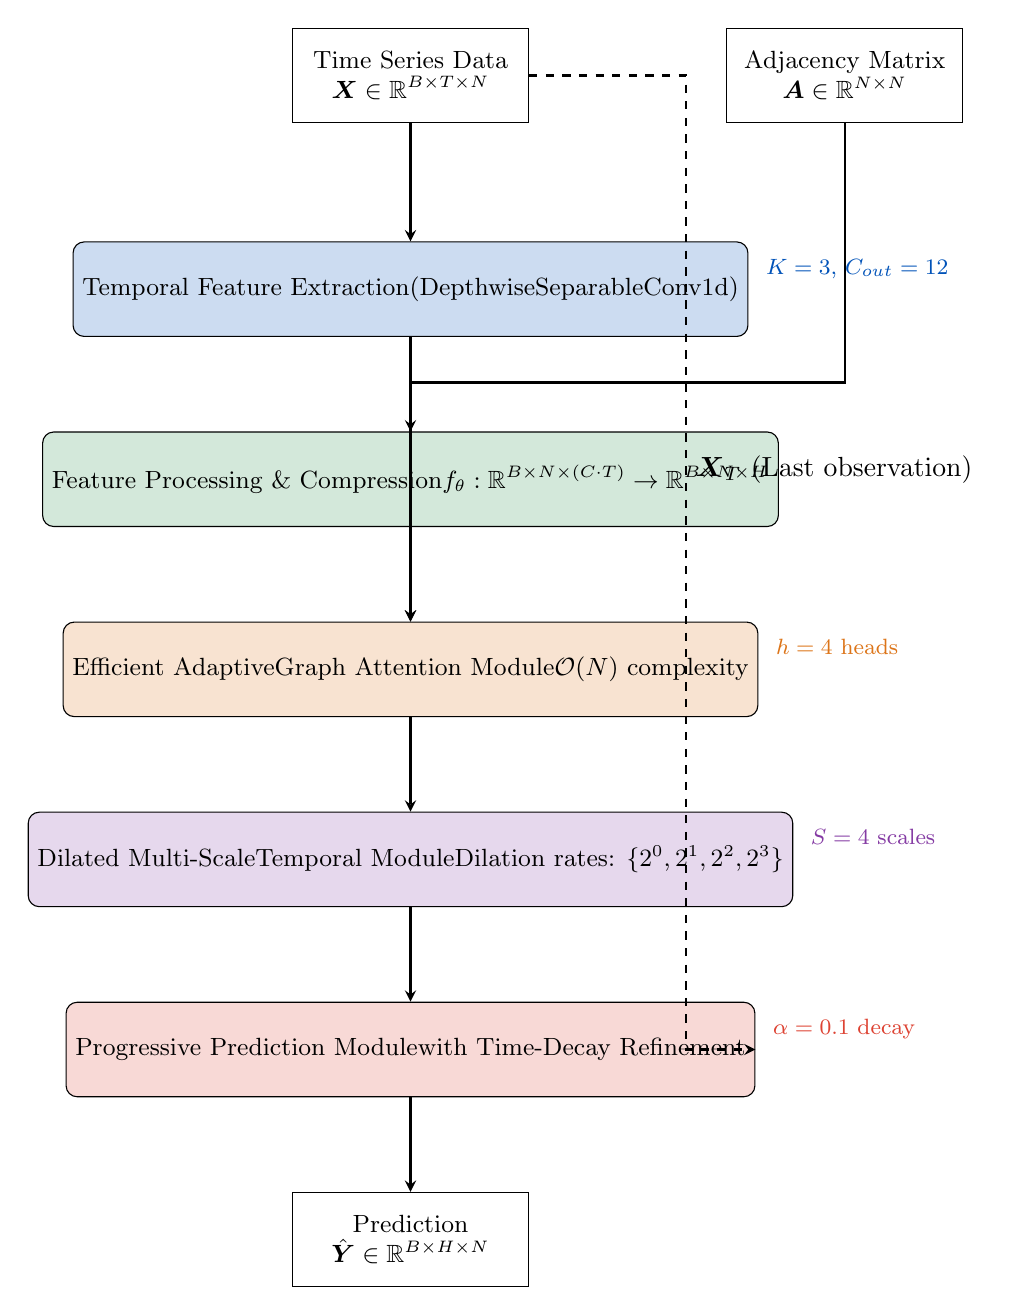
\begin{tikzpicture}[
    node distance=2cm,
    box/.style={rectangle, rounded corners, draw=black, minimum width=3cm, minimum height=1.2cm, text centered, font=\small},
    data/.style={rectangle, draw=black, minimum width=3cm, minimum height=1.2cm, text centered, align=center, font=\small},
    arrow/.style={thick,->,>=stealth}
]

% Input
\node[data] (input) {Time Series Data\\$\boldsymbol{X} \in \mathbb{R}^{B \times T \times N}$};
\node[data, right=2.5cm of input] (adj) {Adjacency Matrix\\$\boldsymbol{A} \in \mathbb{R}^{N \times N}$};

% Feature extraction
\node[box, below=1.5cm of input, fill=myblue!20] (temporal) {Temporal Feature Extraction\\(DepthwiseSeparableConv1d)};

% Feature processing
\node[box, below=1.2cm of temporal, fill=mygreen!20] (processing) {Feature Processing \& Compression\\$f_{\theta}: \mathbb{R}^{B \times N \times (C \cdot T)} \rightarrow \mathbb{R}^{B \times N \times H}$};

% Main components
\node[box, below=1.2cm of processing, fill=myorange!20] (graph) {Efficient Adaptive\\ Graph Attention Module\\$\mathcal{O}(N)$ complexity};
\node[box, below=1.2cm of graph, fill=mypurple!20] (multi) {Dilated Multi-Scale\\ Temporal Module\\Dilation rates: $\{2^0, 2^1, 2^2, 2^3\}$};
\node[box, below=1.2cm of multi, fill=myred!20] (prediction) {Progressive Prediction Module\\with Time-Decay Refinement};

% Output
\node[data, below=1.2cm of prediction] (output) {Prediction\\$\hat{\boldsymbol{Y}} \in \mathbb{R}^{B \times H \times N}$};

% Arrows
\draw[arrow] (input) -- (temporal);
\draw[arrow] (adj) -- ++(0,-3.9) -| (graph);
\draw[arrow] (temporal) -- (processing);
\draw[arrow] (processing) -- (graph);
\draw[arrow] (graph) -- (multi);
\draw[arrow] (multi) -- (prediction);
\draw[arrow] (prediction) -- (output);

% Last observed value connection
\draw[arrow, dashed] (input) -- ++(3.5,0) |- (prediction);
\node[right] at ($(input)+(3.5,-5)$) {$\boldsymbol{X}_{T}$ (Last observation)};

% Module parameters
\node[text=myblue, font=\footnotesize, below right=0.1cm and 0.1cm of temporal.north east] {$K = 3$, $C_{out} = 12$};
\node[text=myorange, font=\footnotesize, below right=0.1cm and 0.1cm of graph.north east] {$h=4$ heads};
\node[text=mypurple, font=\footnotesize, below right=0.1cm and 0.1cm of multi.north east] {$S=4$ scales};
\node[text=myred, font=\footnotesize, below right=0.1cm and 0.1cm of prediction.north east] {$\alpha=0.1$ decay};

\end{tikzpicture}
\caption{Overall architecture of MSAGAT-Net for spatiotemporal forecasting. The model processes time series data $\boldsymbol{X} \in \mathbb{R}^{B \times T \times N}$ and an adjacency matrix $\boldsymbol{A} \in \mathbb{R}^{N \times N}$ through specialized modules for temporal and spatial feature extraction. $B$ represents batch size, $T$ is the input window size, $N$ is the number of nodes, $H$ is the hidden dimension, and the output $\hat{\boldsymbol{Y}}$ provides predictions for the next $H$ time steps.}
\end{figure}

\section{Key Architectural Components}

\subsection{Depthwise Separable Convolution for Temporal Feature Extraction}

\begin{figure}[h]
\centering
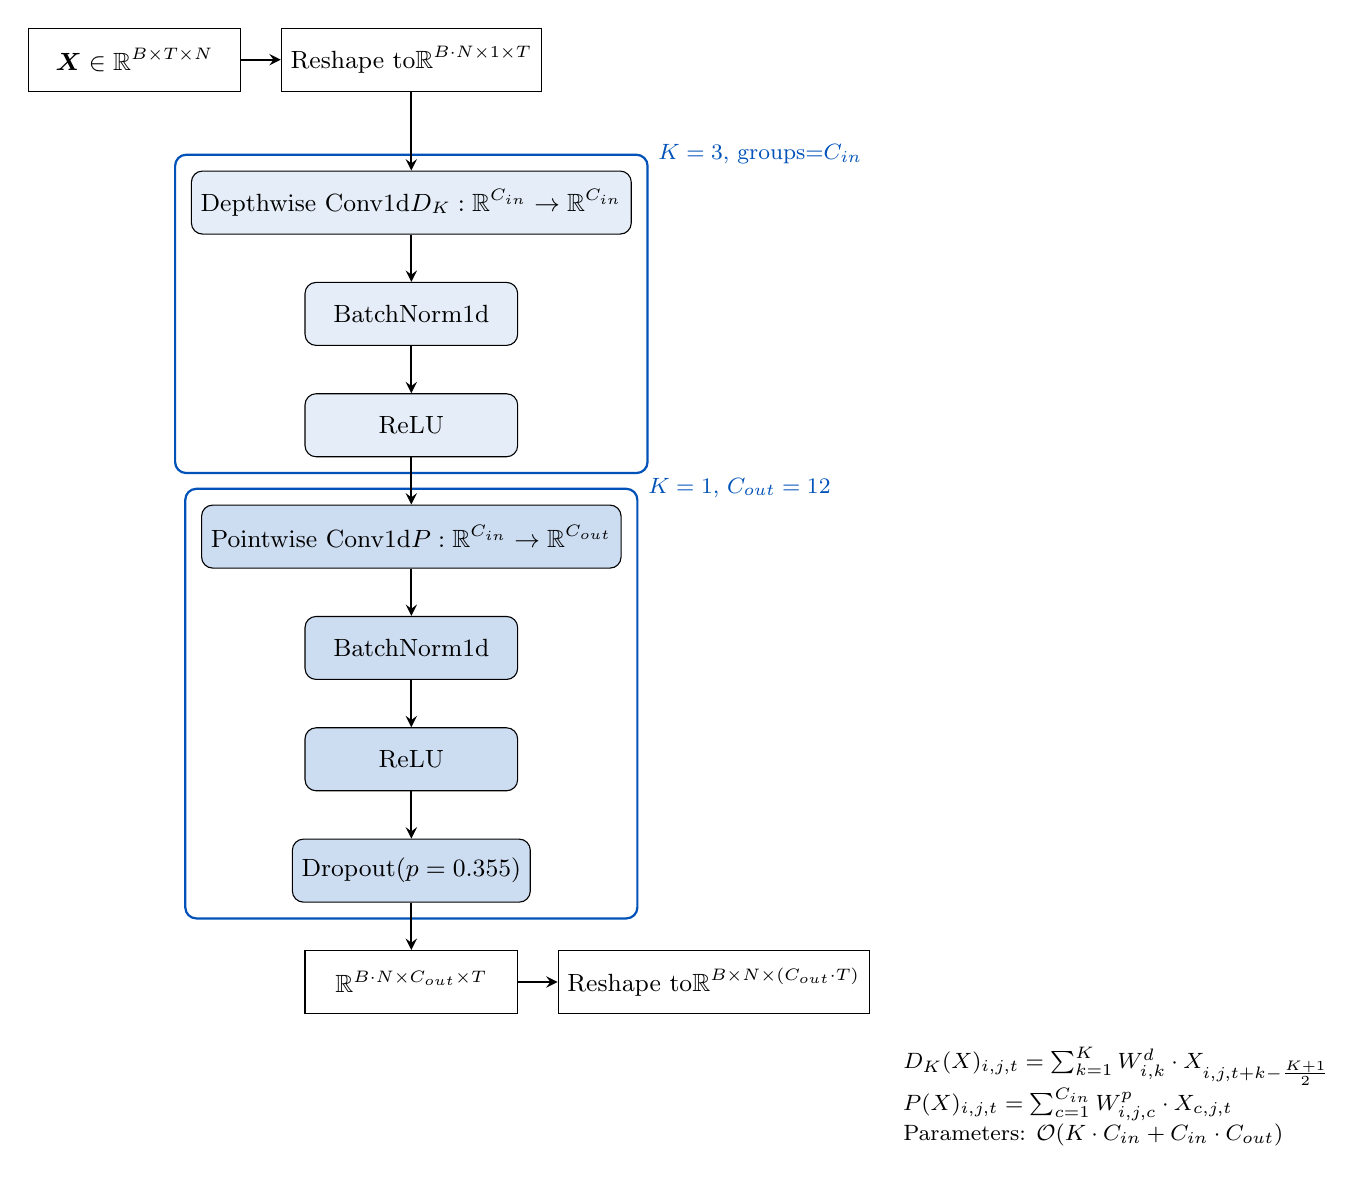
\begin{tikzpicture}[
    node distance=1.8cm,
    box/.style={rectangle, rounded corners, draw=black, minimum width=2.7cm, minimum height=0.8cm, text centered, font=\small},
    data/.style={rectangle, draw=black, minimum width=2.7cm, minimum height=0.8cm, text centered, font=\small},
    arrow/.style={thick,->,>=stealth}
]

% Input and reshape explanation
\node[data] (input) {$\boldsymbol{X} \in \mathbb{R}^{B \times T \times N}$};
\node[data, right=0.5cm of input] (reshape_in) {Reshape to\\$\mathbb{R}^{B \cdot N \times 1 \times T}$};

% Depthwise
\node[box, fill=myblue!10, below=1cm of reshape_in] (depthwise) {Depthwise Conv1d\\$D_{K}: \mathbb{R}^{C_{in}} \rightarrow \mathbb{R}^{C_{in}}$};
\node[box, fill=myblue!10, below=0.6cm of depthwise] (bn1) {BatchNorm1d};
\node[box, fill=myblue!10, below=0.6cm of bn1] (relu1) {ReLU};

% Pointwise
\node[box, fill=myblue!20, below=0.6cm of relu1] (pointwise) {Pointwise Conv1d\\$P: \mathbb{R}^{C_{in}} \rightarrow \mathbb{R}^{C_{out}}$};
\node[box, fill=myblue!20, below=0.6cm of pointwise] (bn2) {BatchNorm1d};
\node[box, fill=myblue!20, below=0.6cm of bn2] (relu2) {ReLU};
\node[box, fill=myblue!20, below=0.6cm of relu2] (dropout) {Dropout($p=0.355$)};

% Output
\node[data, below=0.6cm of dropout] (output) {$\mathbb{R}^{B \cdot N \times C_{out} \times T}$};
\node[data, right=0.5cm of output] (reshape_out) {Reshape to\\$\mathbb{R}^{B \times N \times (C_{out} \cdot T)}$};

% Arrows
\draw[arrow] (input) -- (reshape_in);
\draw[arrow] (reshape_in) -- (depthwise);
\draw[arrow] (depthwise) -- (bn1);
\draw[arrow] (bn1) -- (relu1);
\draw[arrow] (relu1) -- (pointwise);
\draw[arrow] (pointwise) -- (bn2);
\draw[arrow] (bn2) -- (relu2);
\draw[arrow] (relu2) -- (dropout);
\draw[arrow] (dropout) -- (output);
\draw[arrow] (output) -- (reshape_out);

% Group box for depthwise
\begin{pgfonlayer}{background}
\node[rectangle, draw=myblue, thick, inner sep=0.2cm, rounded corners, fit=(depthwise) (relu1)] (depthwise_group) {};
\node[text=myblue, right=0cm of depthwise_group.north east, font=\footnotesize] {$K=3$, groups=$C_{in}$};
\end{pgfonlayer}

% Group box for pointwise
\begin{pgfonlayer}{background}
\node[rectangle, draw=myblue, thick, inner sep=0.2cm, rounded corners, fit=(pointwise) (dropout)] (pointwise_group) {};
\node[text=myblue, right=0cm of pointwise_group.north east, font=\footnotesize] {$K=1$, $C_{out}=12$};
\end{pgfonlayer}

% Mathematical explanation
\node[align=left, anchor=north west, font=\footnotesize] at ($(reshape_out.south east) + (0.3,-0.3)$) {
    $D_K(X)_{i,j,t} = \sum_{k=1}^{K} W^d_{i,k} \cdot X_{i,j,t+k-\frac{K+1}{2}}$\\
    $P(X)_{i,j,t} = \sum_{c=1}^{C_{in}} W^p_{i,j,c} \cdot X_{c,j,t}$\\
    Parameters: $\mathcal{O}(K \cdot C_{in} + C_{in} \cdot C_{out})$
};

\end{tikzpicture}
\caption{Depthwise Separable Convolution for temporal feature extraction. This factorized convolution operation first applies a depthwise convolution $D_K$ with kernel size $K=3$ that processes each channel independently, followed by a pointwise convolution $P$ that mixes the channels. This factorization reduces the parameter count from $\mathcal{O}(K \cdot C_{in} \cdot C_{out})$ to $\mathcal{O}(K \cdot C_{in} + C_{in} \cdot C_{out})$ while maintaining strong representational capacity.}
\end{figure}

\subsection{Efficient Adaptive Graph Attention Module}

\begin{figure}[h]
\centering
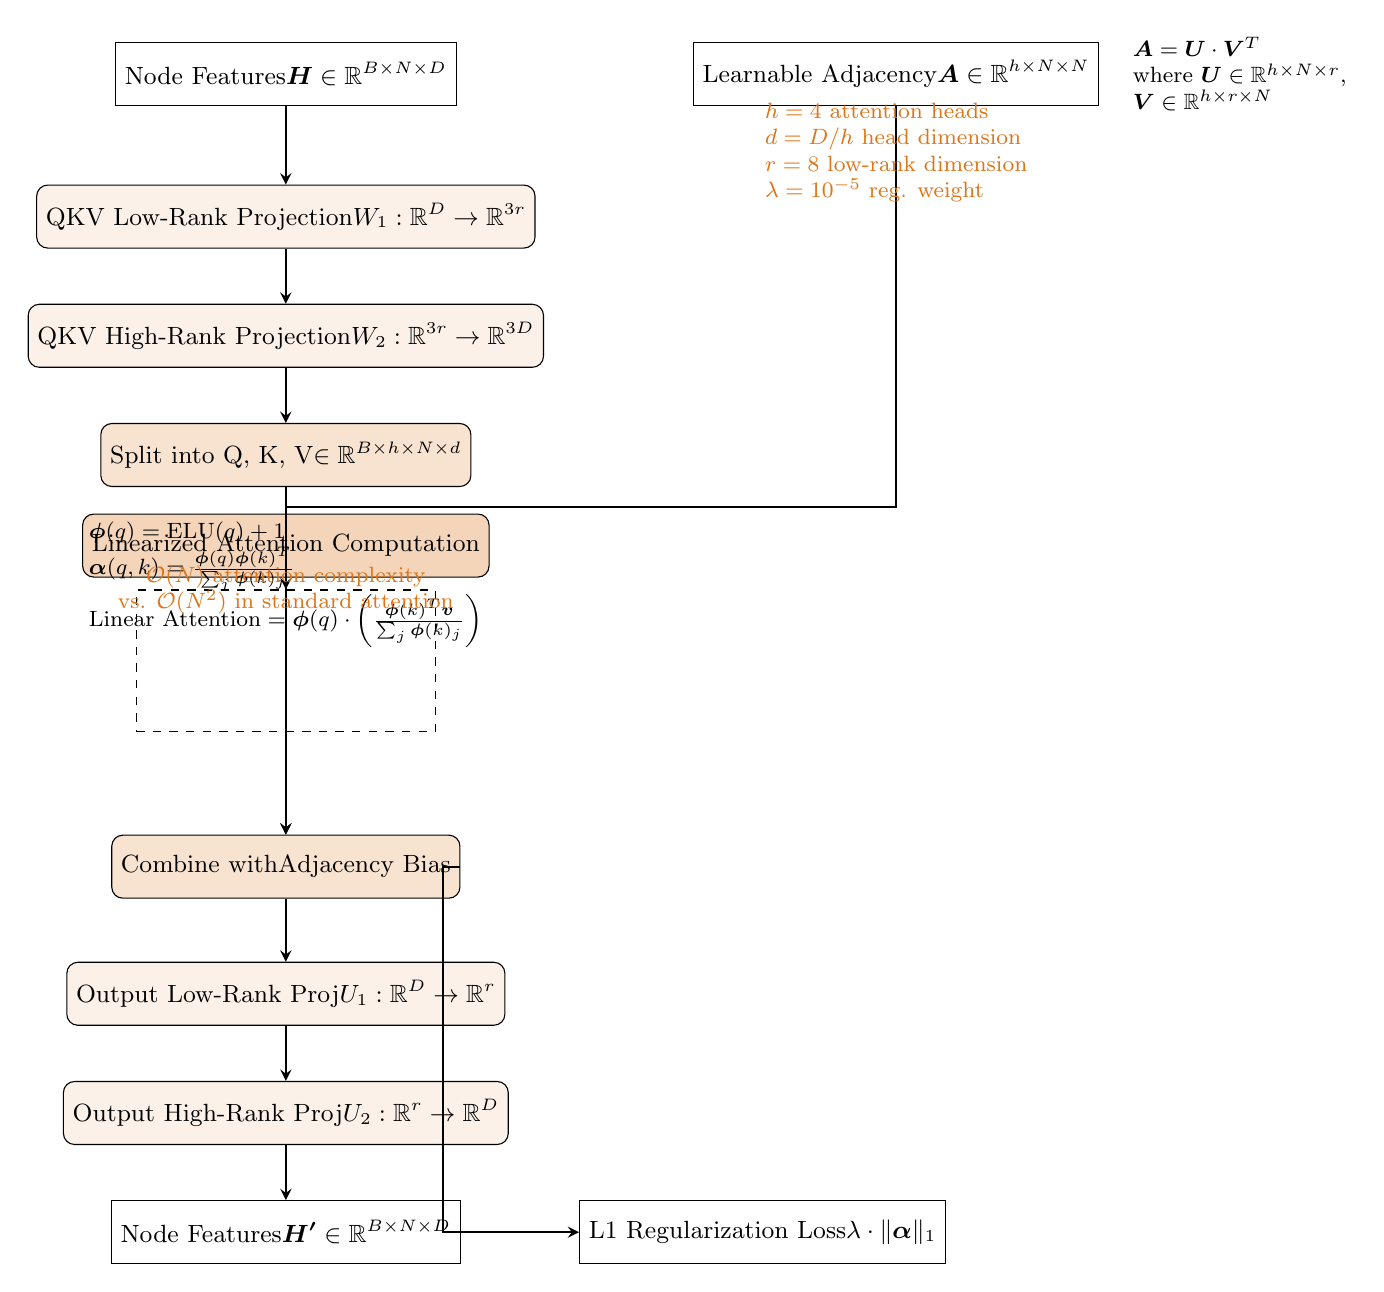
\begin{tikzpicture}[
    node distance=2cm,
    box/.style={rectangle, rounded corners, draw=black, minimum width=3cm, minimum height=0.8cm, text centered, font=\small},
    data/.style={rectangle, draw=black, minimum width=3cm, minimum height=0.8cm, text centered, font=\small},
    proc/.style={rectangle, draw=black, dashed, minimum width=3.8cm, minimum height=1.8cm, text centered},
    arrow/.style={thick,->,>=stealth}
]

% Input
\node[data] (input) {Node Features\\$\boldsymbol{H} \in \mathbb{R}^{B \times N \times D}$};
\node[data, right=3cm of input] (adj) {Learnable Adjacency\\$\boldsymbol{A} \in \mathbb{R}^{h \times N \times N}$};

% Low-rank projection
\node[box, fill=myorange!10, below=1cm of input] (qkv_low) {QKV Low-Rank Projection\\$W_1: \mathbb{R}^{D} \rightarrow \mathbb{R}^{3r}$};
\node[box, fill=myorange!10, below=0.7cm of qkv_low] (qkv_high) {QKV High-Rank Projection\\$W_2: \mathbb{R}^{3r} \rightarrow \mathbb{R}^{3D}$};

% QKV separation
\node[box, fill=myorange!20, below=0.7cm of qkv_high] (qkv_split) {Split into Q, K, V\\$\in \mathbb{R}^{B \times h \times N \times d}$};

% Attention computation
\node[proc, below=1.3cm of qkv_split] (attn_comp) {};
\node[box, fill=myorange!30, above=0.15cm of attn_comp.north] (linear_attn) {Linearized Attention Computation};

% Combine with adjacency
\node[box, fill=myorange!20, below=1.3cm of attn_comp] (combine) {Combine with\\Adjacency Bias};

% Output projection
\node[box, fill=myorange!10, below=0.8cm of combine] (out_low) {Output Low-Rank Proj\\$U_1: \mathbb{R}^{D} \rightarrow \mathbb{R}^{r}$};
\node[box, fill=myorange!10, below=0.7cm of out_low] (out_high) {Output High-Rank Proj\\$U_2: \mathbb{R}^{r} \rightarrow \mathbb{R}^{D}$};

% Output
\node[data, below=0.7cm of out_high] (output) {Node Features\\$\boldsymbol{H'} \in \mathbb{R}^{B \times N \times D}$};
\node[data, right=1.5cm of output] (reg_loss) {L1 Regularization Loss\\$\lambda \cdot \|\boldsymbol{\alpha}\|_1$};

% Arrows
\draw[arrow] (input) -- (qkv_low);
\draw[arrow] (qkv_low) -- (qkv_high);
\draw[arrow] (qkv_high) -- (qkv_split);
\draw[arrow] (qkv_split) -- (attn_comp);
\draw[arrow] (adj) -- ++(0,-5.5) -| (combine);
\draw[arrow] (attn_comp) -- (combine);
\draw[arrow] (combine) -- (out_low);
\draw[arrow] (out_low) -- (out_high);
\draw[arrow] (out_high) -- (output);
\draw[arrow] (combine) -- ++(2,0) |- (reg_loss);

% Mathematical details
\node[align=left, font=\footnotesize] at ($(linear_attn) + (0,-0.5)$) {
    $\boldsymbol{\phi}(q) = \text{ELU}(q) + 1$\\
    $\boldsymbol{\alpha}(q,k) = \frac{\boldsymbol{\phi}(q)\boldsymbol{\phi}(k)^T}{\sum_j \boldsymbol{\phi}(k)_j}$\\
    $\text{Linear Attention} = \boldsymbol{\phi}(q) \cdot \left(\frac{\boldsymbol{\phi}(k)^T \boldsymbol{v}}{\sum_j \boldsymbol{\phi}(k)_j}\right)$
};

% Label for attention complexity
\node[text=myorange, align=center, font=\footnotesize] at ($(attn_comp) + (0,0.9)$) {$\mathcal{O}(N)$ attention complexity\\vs. $\mathcal{O}(N^2)$ in standard attention};

% Parameters
\node[text=myorange, align=left, font=\footnotesize] at ($(adj) + (0,-1)$) {
    $h=4$ attention heads\\
    $d=D/h$ head dimension\\
    $r=8$ low-rank dimension\\
    $\lambda=10^{-5}$ reg. weight
};

% Factorization explanation
\node[align=left, anchor=west, font=\footnotesize] at ($(adj.east) + (0.3,0)$) {
    $\boldsymbol{A} = \boldsymbol{U} \cdot \boldsymbol{V}^T$\\
    where $\boldsymbol{U} \in \mathbb{R}^{h \times N \times r}$,\\
    $\boldsymbol{V} \in \mathbb{R}^{h \times r \times N}$
};

\end{tikzpicture}
\caption{Efficient Adaptive Graph Attention Module with $\mathcal{O}(N)$ complexity and low-rank factorization. This module implements linear attention using the ELU+1 kernel trick, which transforms the quadratic complexity of standard attention to linear. The learnable adjacency matrix is factorized as $\boldsymbol{A} = \boldsymbol{U} \cdot \boldsymbol{V}^T$ to reduce memory requirements from $\mathcal{O}(N^2)$ to $\mathcal{O}(Nr)$. All projection matrices are decomposed using low-rank factorization for parameter efficiency. The L1 regularization encourages sparse attention patterns for better interpretability.}
\end{figure}

\subsection{Dilated Multi-Scale Temporal Module}

\begin{figure}[h]
\centering
\begin{tikzpicture}[
    node distance=1.5cm,
    box/.style={rectangle, rounded corners, draw=black, minimum width=2.8cm, minimum height=0.8cm, text centered, font=\small},
    data/.style={rectangle, draw=black, minimum width=2.8cm, minimum height=0.8cm, text centered, font=\small},
    scale/.style={rectangle, draw=black, rounded corners, fill=mypurple!10, minimum width=2.8cm, minimum height=2.2cm, text centered, font=\small},
    arrow/.style={thick,->,>=stealth}
]

% Input
\node[data] (input) {Input Features\\$\boldsymbol{H} \in \mathbb{R}^{B \times N \times D}$};

% Scale modules
\node[scale, below=1.8cm of input, xshift=-4.8cm] (scale1) {Scale 1\\Dilation = $2^0 = 1$\\Conv1d + BN + ReLU\\Receptive field: 3};
\node[scale, right=0.5cm of scale1] (scale2) {Scale 2\\Dilation = $2^1 = 2$\\Conv1d + BN + ReLU\\Receptive field: 5};
\node[scale, right=0.5cm of scale2] (scale3) {Scale 3\\Dilation = $2^2 = 4$\\Conv1d + BN + ReLU\\Receptive field: 9};
\node[scale, right=0.5cm of scale3] (scale4) {Scale 4\\Dilation = $2^3 = 8$\\Conv1d + BN + ReLU\\Receptive field: 17};

% Fusion
\node[box, fill=mypurple!30, below=1.8cm of input] (fusion) {Adaptive Scale Fusion\\$\boldsymbol{\alpha} = \text{softmax}(\boldsymbol{w})$};
\node[box, fill=mypurple!20, below=0.7cm of fusion] (fusion_low) {Fusion Low-Rank Proj\\$\mathbb{R}^{D} \rightarrow \mathbb{R}^{r}$};
\node[box, fill=mypurple!20, below=0.7cm of fusion_low] (fusion_high) {Fusion High-Rank Proj\\$\mathbb{R}^{r} \rightarrow \mathbb{R}^{D}$};
\node[box, fill=mypurple!20, below=0.7cm of fusion_high] (layernorm) {LayerNorm + Residual};

% Output
\node[data, below=0.7cm of layernorm] (output) {Output Features\\$\boldsymbol{H'} \in \mathbb{R}^{B \times N \times D}$};

% Arrows with patterns
\draw[arrow] (input) -- ++(0,-0.9) -| (scale1.north);
\draw[arrow] (input) -- ++(0,-0.9) -| (scale2.north);
\draw[arrow] (input) -- ++(0,-0.9) -| (scale3.north);
\draw[arrow] (input) -- ++(0,-0.9) -| (scale4.north);

\draw[arrow] (scale1.south) -- ++(0,-0.5) -| (fusion.north);
\draw[arrow] (scale2.south) -- ++(0,-0.5) -| (fusion.north);
\draw[arrow] (scale3.south) -- ++(0,-0.5) -| (fusion.north);
\draw[arrow] (scale4.south) -- ++(0,-0.5) -| (fusion.north);

\draw[arrow] (fusion) -- (fusion_low);
\draw[arrow] (fusion_low) -- (fusion_high);
\draw[arrow] (fusion_high) -- (layernorm);
\draw[arrow] (layernorm) -- (output);

% Residual connection
\draw[arrow, dashed] (fusion) -- ++(3.5,0) |- (layernorm);

% Mathematical details
\node[align=left, anchor=west, font=\footnotesize] at ($(scale4.east) + (0.5,0)$) {
    $\boldsymbol{F}_i = \text{Conv1d}(\boldsymbol{H}, d=2^{i-1})$\\
    $\boldsymbol{F}_{\text{fused}} = \sum_{i=1}^{S} \alpha_i \boldsymbol{F}_i$\\
    where $\boldsymbol{\alpha} = \text{softmax}(\boldsymbol{w})$\\
    $\boldsymbol{w} \in \mathbb{R}^S$ are learnable weights\\
    $S=4$ is the number of scales
};

\end{tikzpicture}
\caption{Dilated Multi-Scale Temporal Module with adaptive fusion of features from different time scales. This module captures temporal patterns at multiple resolutions by using parallel dilated convolutions with exponentially increasing dilation rates (1, 2, 4, 8). This creates an effective receptive field ranging from 3 to 17 time steps without requiring deep stacking of layers. The features from different scales are combined using learned weights that are dynamically adapted during training. A residual connection helps maintain gradient flow.}
\end{figure}

\subsection{Progressive Prediction Module}

\begin{figure}[h]
\centering
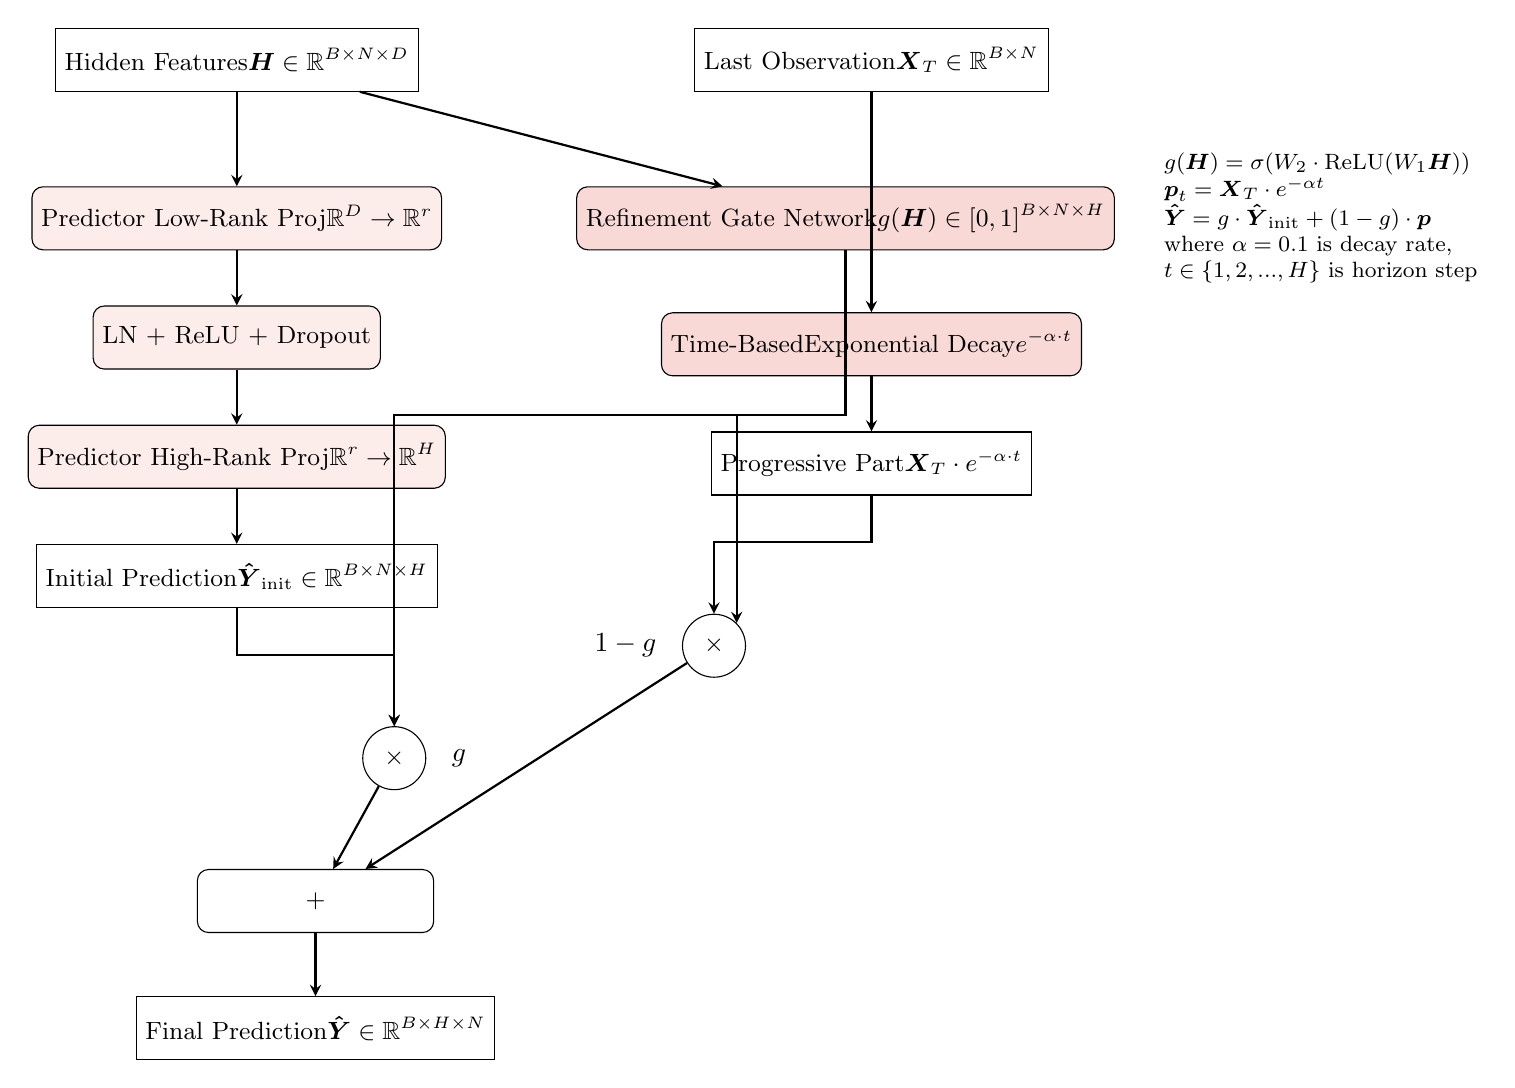
\begin{tikzpicture}[
    node distance=1.5cm,
    box/.style={rectangle, rounded corners, draw=black, minimum width=3cm, minimum height=0.8cm, text centered, font=\small},
    data/.style={rectangle, draw=black, minimum width=3cm, minimum height=0.8cm, text centered, font=\small},
    gate/.style={circle, draw=black, minimum size=0.8cm, text centered, font=\small},
    arrow/.style={thick,->,>=stealth}
]

% Inputs
\node[data] (input) {Hidden Features\\$\boldsymbol{H} \in \mathbb{R}^{B \times N \times D}$};
\node[data, right=3.5cm of input] (last) {Last Observation\\$\boldsymbol{X}_T \in \mathbb{R}^{B \times N}$};

% Prediction pathway
\node[box, fill=myred!10, below=1.2cm of input] (pred_low) {Predictor Low-Rank Proj\\$\mathbb{R}^{D} \rightarrow \mathbb{R}^{r}$};
\node[box, fill=myred!10, below=0.7cm of pred_low] (pred_mid) {LN + ReLU + Dropout};
\node[box, fill=myred!10, below=0.7cm of pred_mid] (pred_high) {Predictor High-Rank Proj\\$\mathbb{R}^{r} \rightarrow \mathbb{R}^{H}$};
\node[data, below=0.7cm of pred_high] (init_pred) {Initial Prediction\\$\boldsymbol{\hat{Y}}_{\text{init}} \in \mathbb{R}^{B \times N \times H}$};

% Refinement pathway
\node[box, fill=myred!20, below right=1.2cm and 2cm of input] (refine_gate) {Refinement Gate Network\\$g(\boldsymbol{H}) \in [0,1]^{B \times N \times H}$};
\node[box, fill=myred!20, below=2.8cm of last] (time_decay) {Time-Based\\Exponential Decay\\$e^{-\alpha \cdot t}$};
\node[data, below=0.7cm of time_decay] (prog_part) {Progressive Part\\$\boldsymbol{X}_T \cdot e^{-\alpha \cdot t}$};

% Gating mechanism
\node[gate, below=1.5cm of init_pred, xshift=2cm] (gate) {$\times$};
\node[gate, below=1.5cm of prog_part, xshift=-2cm] (gate2) {$\times$};
\node[box, below=1cm of gate, xshift=-1cm] (add) {$+$};

% Output
\node[data, below=0.8cm of add] (output) {Final Prediction\\$\boldsymbol{\hat{Y}} \in \mathbb{R}^{B \times H \times N}$};

% Arrows
\draw[arrow] (input) -- (pred_low);
\draw[arrow] (pred_low) -- (pred_mid);
\draw[arrow] (pred_mid) -- (pred_high);
\draw[arrow] (pred_high) -- (init_pred);

\draw[arrow] (input) -- (refine_gate);
\draw[arrow] (last) -- (time_decay);
\draw[arrow] (time_decay) -- (prog_part);

\draw[arrow] (init_pred) -- ++(0,-1) -| (gate);
\draw[arrow] (refine_gate) -- ++(0,-2.5) -| (gate);
\draw[arrow] (refine_gate) -- ++(0,-2.5) -| (gate2.north east);
\draw[arrow] (prog_part) -- ++(0,-1) -| (gate2);

\draw[arrow] (gate) -- (add);
\draw[arrow] (gate2) -- (add);
\draw[arrow] (add) -- (output);

% Gate labels
\node[right=0.2cm of gate] {$g$};
\node[left=0.2cm of gate2] {$1-g$};

% Mathematical formulation
\node[align=left, anchor=west, font=\footnotesize] at ($(refine_gate.east) + (0.5,0)$) {
    $g(\boldsymbol{H}) = \sigma(W_2 \cdot \text{ReLU}(W_1 \boldsymbol{H}))$\\
    $\boldsymbol{p}_t = \boldsymbol{X}_T \cdot e^{-\alpha t}$\\
    $\boldsymbol{\hat{Y}} = g \cdot \boldsymbol{\hat{Y}}_{\text{init}} + (1-g) \cdot \boldsymbol{p}$\\
    where $\alpha=0.1$ is decay rate,\\
    $t \in \{1,2,...,H\}$ is horizon step
};

\end{tikzpicture}
\caption{Progressive Prediction Module with adaptive gating and time-decay refinement. This module generates initial multi-step predictions that are then adaptively combined with a persistence forecast derived from the last observation $\boldsymbol{X}_T$. The gating network dynamically determines how much to rely on the model's prediction versus the persistence forecast for each node and time step. The persistence forecast is adjusted with an exponential decay factor $e^{-\alpha t}$ to reflect decreasing confidence in persistent patterns over longer horizons. This approach helps stabilize predictions, especially for shorter horizons.}
\end{figure}

\section{Tensor Flow Throughout Network}

\begin{figure}[h]
\centering
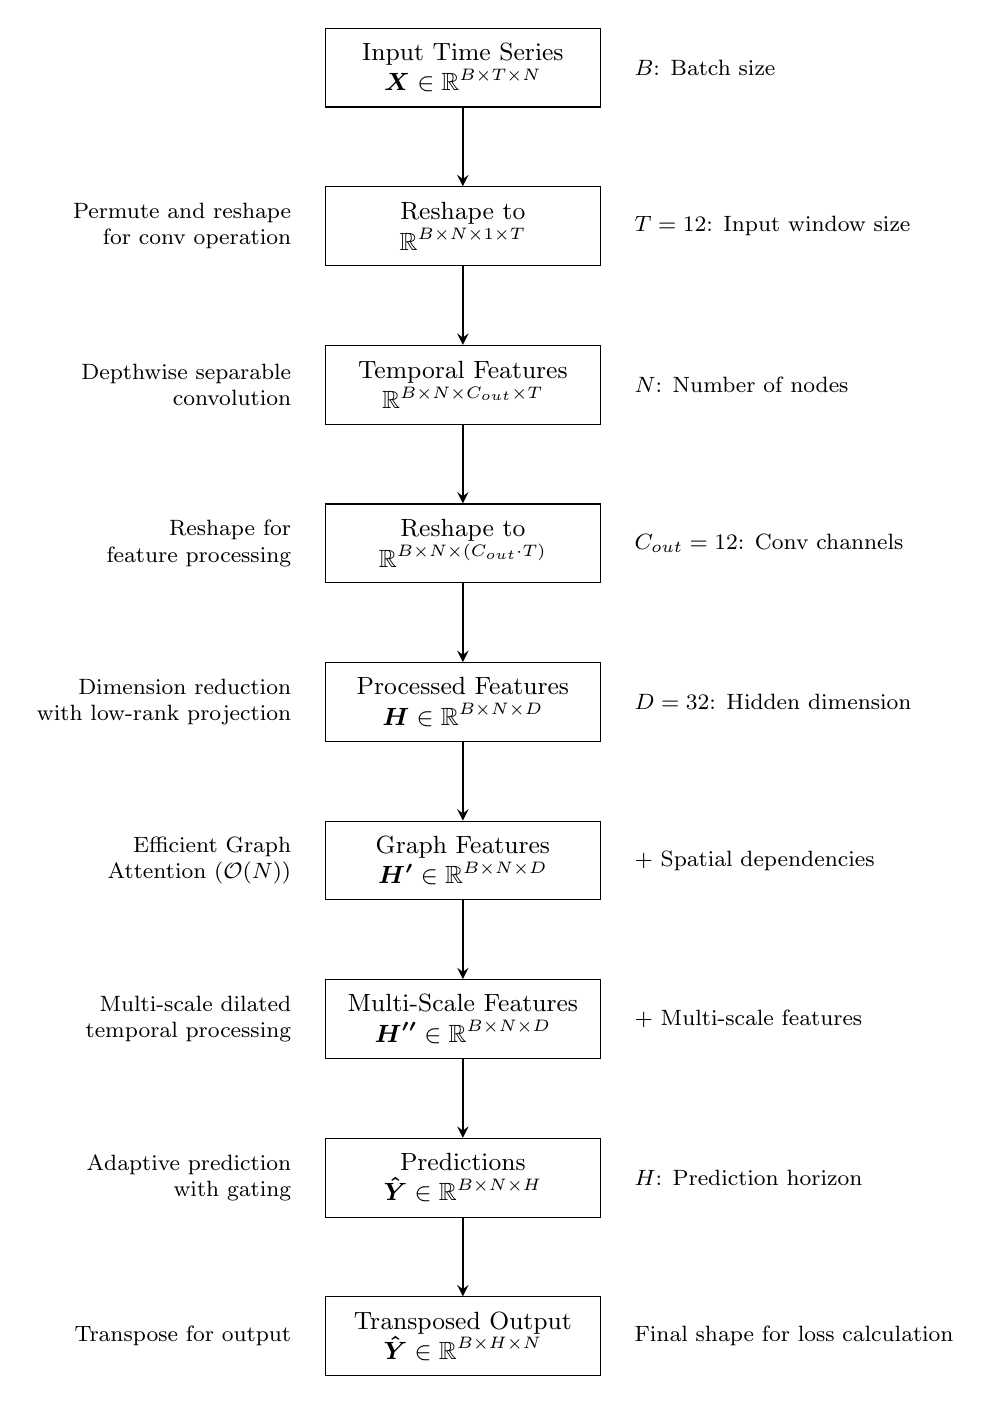
\begin{tikzpicture}[
    node distance=2cm,
    data/.style={rectangle, draw=black, minimum width=3.5cm, minimum height=1cm, text centered, align=center, font=\small},
    arrow/.style={thick,->,>=stealth}
]

% Input format
\node[data] (input) {Input Time Series\\$\boldsymbol{X} \in \mathbb{R}^{B \times T \times N}$};

% Data reshaping
\node[data, below=1cm of input] (reshape) {Reshape to\\$\mathbb{R}^{B \times N \times 1 \times T}$};

% Temporal features
\node[data, below=1cm of reshape] (temp_feat) {Temporal Features\\$\mathbb{R}^{B \times N \times C_{out} \times T}$};

% Reshaping back
\node[data, below=1cm of temp_feat] (reshape2) {Reshape to\\$\mathbb{R}^{B \times N \times (C_{out} \cdot T)}$};

% Feature processing
\node[data, below=1cm of reshape2] (process) {Processed Features\\$\boldsymbol{H} \in \mathbb{R}^{B \times N \times D}$};

% Graph features
\node[data, below=1cm of process] (graph) {Graph Features\\$\boldsymbol{H'} \in \mathbb{R}^{B \times N \times D}$};

% Temporal fusion
\node[data, below=1cm of graph] (temporal) {Multi-Scale Features\\$\boldsymbol{H''} \in \mathbb{R}^{B \times N \times D}$};

% Prediction
\node[data, below=1cm of temporal] (pred) {Predictions\\$\boldsymbol{\hat{Y}} \in \mathbb{R}^{B \times N \times H}$};

% Output
\node[data, below=1cm of pred] (output) {Transposed Output\\$\boldsymbol{\hat{Y}} \in \mathbb{R}^{B \times H \times N}$};

% Arrows
\draw[arrow] (input) -- (reshape);
\draw[arrow] (reshape) -- (temp_feat);
\draw[arrow] (temp_feat) -- (reshape2);
\draw[arrow] (reshape2) -- (process);
\draw[arrow] (process) -- (graph);
\draw[arrow] (graph) -- (temporal);
\draw[arrow] (temporal) -- (pred);
\draw[arrow] (pred) -- (output);

% Dimension labels
\node[anchor=west, font=\footnotesize] at ($(input.east) + (0.3,0)$) {$B$: Batch size};
\node[anchor=west, font=\footnotesize] at ($(reshape.east) + (0.3,0)$) {$T=12$: Input window size};
\node[anchor=west, font=\footnotesize] at ($(temp_feat.east) + (0.3,0)$) {$N$: Number of nodes};
\node[anchor=west, font=\footnotesize] at ($(reshape2.east) + (0.3,0)$) {$C_{out}=12$: Conv channels};
\node[anchor=west, font=\footnotesize] at ($(process.east) + (0.3,0)$) {$D=32$: Hidden dimension};
\node[anchor=west, font=\footnotesize] at ($(graph.east) + (0.3,0)$) {+ Spatial dependencies};
\node[anchor=west, font=\footnotesize] at ($(temporal.east) + (0.3,0)$) {+ Multi-scale features};
\node[anchor=west, font=\footnotesize] at ($(pred.east) + (0.3,0)$) {$H$: Prediction horizon};
\node[anchor=west, font=\footnotesize] at ($(output.east) + (0.3,0)$) {Final shape for loss calculation};

% Operations
\node[anchor=east, align=right, font=\footnotesize] at ($(reshape.west) + (-0.3,0)$) {Permute and reshape\\for conv operation};
\node[anchor=east, align=right, font=\footnotesize] at ($(temp_feat.west) + (-0.3,0)$) {Depthwise separable\\convolution};
\node[anchor=east, align=right, font=\footnotesize] at ($(reshape2.west) + (-0.3,0)$) {Reshape for\\feature processing};
\node[anchor=east, align=right, font=\footnotesize] at ($(process.west) + (-0.3,0)$) {Dimension reduction\\with low-rank projection};
\node[anchor=east, align=right, font=\footnotesize] at ($(graph.west) + (-0.3,0)$) {Efficient Graph\\Attention ($\mathcal{O}(N)$)};
\node[anchor=east, align=right, font=\footnotesize] at ($(temporal.west) + (-0.3,0)$) {Multi-scale dilated\\temporal processing};
\node[anchor=east, align=right, font=\footnotesize] at ($(pred.west) + (-0.3,0)$) {Adaptive prediction\\with gating};
\node[anchor=east, align=right, font=\footnotesize] at ($(output.west) + (-0.3,0)$) {Transpose for output};

\end{tikzpicture}
\caption{Detailed tensor flow through the MSAGAT-Net architecture showing dimensions and transformations at each stage. The network processes input time series data with shape $[B, T, N]$ through a sequence of specialized modules that extract and combine temporal and spatial features. Low-rank projections are used throughout the network to reduce parameters while maintaining model capacity. The final output tensor $[B, H, N]$ provides predictions for each node across the forecast horizon.}
\end{figure}

\section{Mathematical Formulation}

The MSAGAT-Net model can be described mathematically as follows:

\begin{align}
\boldsymbol{X} &\in \mathbb{R}^{B \times T \times N} &\text{(Input time series)} \\
\boldsymbol{A} &\in \mathbb{R}^{N \times N} &\text{(Adjacency matrix)} \\
\boldsymbol{F} &= \text{TemporalFeatureExtraction}(\boldsymbol{X}) &\text{(Temporal features)} \\
\boldsymbol{H} &= \text{FeatureProcessing}(\boldsymbol{F}) &\text{(Processed features)} \\
\boldsymbol{H'} &= \text{EfficientGraphAttention}(\boldsymbol{H}, \boldsymbol{A}) &\text{(Spatial features)} \\
\boldsymbol{H''} &= \text{MultiScaleTemporal}(\boldsymbol{H'}) &\text{(Multi-scale features)} \\
\boldsymbol{\hat{Y}} &= \text{ProgressivePrediction}(\boldsymbol{H''}, \boldsymbol{X}_T) &\text{(Predictions)} \\
\mathcal{L} &= \text{MSE}(\boldsymbol{Y}, \boldsymbol{\hat{Y}}) + \lambda \|\boldsymbol{\alpha}\|_1 &\text{(Loss function)}
\end{align}

where $\boldsymbol{X}_T$ represents the last observed values and $\lambda \|\boldsymbol{\alpha}\|_1$ is the attention regularization term that encourages sparse attention patterns for better interpretability.

\end{document}